\documentclass[12pt]{article}
%\usepackage{alltt}
%\usepackage{helvet}
%\usepackage[sfdefault]{roboto}
\usepackage{amsmath}
\usepackage[utf8]{inputenc}
\usepackage[dvips]{graphicx}
%\usepackage{a4wide}
\usepackage{epsfig}
\usepackage{fancybox}
\usepackage{verbatim}
\usepackage{array}
\usepackage{latexsym}
\usepackage{alltt}
\usepackage{url}
\usepackage{color}   % added for colored text
%\usepackage{fullpage}
\usepackage{hyperref}
\usepackage{listings}
\usepackage{color}
\usepackage{calc}
\usepackage{enumitem}
\usepackage[hmargin=3cm,vmargin=5.0cm]{geometry}
%\topmargin=0cm
\topmargin=-1.8cm \addtolength{\textheight}{4.5cm}
\addtolength{\textwidth}{1.0cm}
%\setlength{\leftmargin}{-5cm}
\setlength{\oddsidemargin}{0.0cm}
\setlength{\evensidemargin}{0.0cm}

%\renewcommand{\familydefault}{\sfdefault}

\newcommand{\HRule}{\rule{\linewidth}{1mm}}
\newcommand{\kutu}[2]{\framebox[#1mm]{\rule[-2mm]{0mm}{#2mm}}}
\newcommand{\gap}{ \\[1mm] }

\newcommand{\Q}{\raisebox{1.7pt}{$\scriptstyle\bigcirc$}}

\definecolor{amaranth}{rgb}{0.9, 0.17, 0.31}
\definecolor{gray}{rgb}{0.4,0.4,0.4}
\definecolor{darkblue}{rgb}{0.0,0.0,0.6}
\definecolor{cyan}{rgb}{0.0,0.6,0.6}
\definecolor{red}{rgb}{0.6,0,0}
\definecolor{dkgreen}{rgb}{0,0.6,0}
\definecolor{mauve}{rgb}{0.58,0,0.82}
\definecolor{lightblue}{rgb}{0.0,0.0,0.9}
\definecolor{darkred}{rgb}{0.6,0.0,0.0}

\lstset{
    %backgroundcolor=\color{lbcolor},
    tabsize=4,
    basicstyle=\fontsize{10}{10.3}\selectfont\sffamily,
    numberstyle=\footnotesize,
    aboveskip={0.0\baselineskip},
    belowskip={0.0\baselineskip},
    columns=fullflexible,
    breaklines=true,
    prebreak=\raisebox{0ex}[0ex][0ex]{\ensuremath{\hookleftarrow}},
    frame=single,
    showtabs=false,
    showspaces=false,
    showstringspaces=false,
    identifierstyle=\color{amaranth},
    keywordstyle=\color{rgb}{0,0,1},
    commentstyle=\color[rgb]{0.133,0.545,0.133},
    stringstyle=\color{amaranth},
}

\lstdefinelanguage{XML}
{
  morestring=[s][\color{red}]{"}{"},
  morestring=[s][\color{black}]{>}{<},
  morecomment=[s]{<?}{?>},
  morecomment=[s][\color{dkgreen}]{<!--}{-->},
  %stringstyle=\color{black},
  identifierstyle=\color{black},
  keywordstyle=\color{darkblue},
  commentstyle=\color[rgb]{0.133,0.545,0.133},
  stringstyle=\color{black},
  morekeywords={Scene,BackgroundColor,ShadowRayEpsilon,
  MaxRecursionDepth,Cameras,Camera,Position,Gaze,Up,
  NearPlane,NearDistance,ImageResolution,ImageName,
  Material,Materials,VertexData,Mesh,Triangle,Sphere,
  Faces,Lights,AmbientLight,PointLight,Objects,Indices,
  AmbientReflectance,DiffuseReflectance,SpecularReflectance,PhongExponent,MirrorReflectance,Intensity,Center,Radius,xmlns,version}% list your attributes here
}

\begin{document}

\noindent \HRule \\[3mm]
\small
\begin{tabular}[b]{lp{1.2cm}r}
\href{https://www.metu.edu.tr/}{
\epsfig{file=metulogo.eps,width=5mm}} Middle East Technical
University &  &
\href{https://ceng.metu.edu.tr/information}{
\epsfig{file=bmblogo.eps,width=5mm}} Department of Computer Engineering \\
\end{tabular} \\
\begin{center}

                 \LARGE \textbf{CENG 795} \\[4mm]
                 \Large Advanced Ray Tracing \\[4mm]
                \normalsize Fall '2022-2023 \\
                    \normalsize Assignment 5 - Advanced Lighting and HDR Rendering\\
                    \normalsize (v.1.0)
\end{center}
\HRule

\begin{center}
Due date: January 2, 2022, Monday, 23:59
\end{center}

\centerline{
    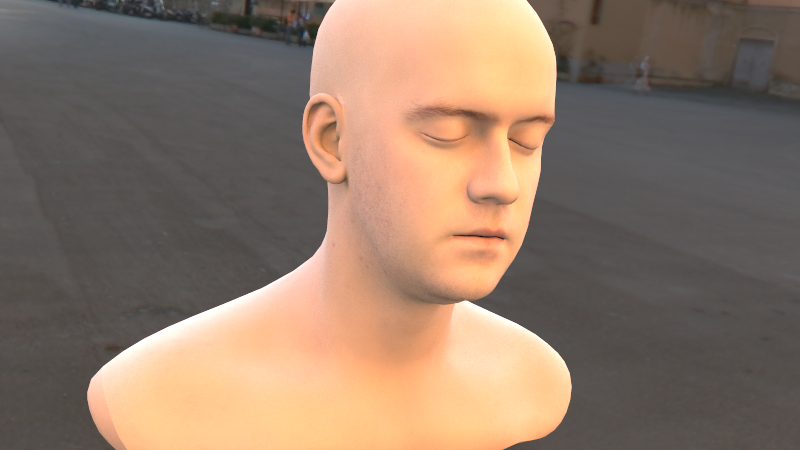
\includegraphics[width=5in]{../outputs/head_env_light.png}
}

\section{Objectives}

In this homework you are going to add new lights to your ray tracers.
Some of these lights can be high dynamic range (HDR) environment maps.
As a result of this, you will no longer save your outputs as PNG files
clipped to $[0, 255]$ range. Instead you will save your results as HDR
images in .exr or .hdr formats. You will also tone map these images and
then save them as PNG images. The following new lights are added:

\begin{itemize}
    \item Directional lights
    \item Spot lights
    \item Environment lights
\end{itemize}

\vspace{0.5cm} \noindent \textbf{Keywords:} \emph{environment mapping, HDR imaging, gamma correction}

\section{Specifications}

The specifications are the same as for the previous
homeworks so are not repeated here. For reading/writing HDR images you
can use a library of your choice. OpenCV has support for HDR images.
There appears to be another library (not tested) called tinyexr that you
can use for this purpose: \url{https://github.com/syoyo/tinyexr}

\section{Scene File}
\label{sec:sceneFile}

\noindent Please see the previous assignments for a detailed
description of the scene file.  In this section, only the elements
introduced in this homework are explained.

\subsection{Camera}

Camera element has now the following added child elements to support
tone mapping:

\begin{verbatim}
<ImageName>output.exr</ImageName>
<Tonemap>
    <TMO>Photographic</TMO>
    <TMOOptions>0.18 1</TMOOptions> <!-- key_value burn_percent -->
    <Saturation>1.0</Saturation>
    <Gamma>2.2</Gamma>
</Tonemap>
\end{verbatim}

ImageName element existed before but now it can contain an HDR file
name. If this is the case (as in output.exr), you must use the following
tone mapping specifications. You are only expected to support the
photographic tone mapping algorithm~\footnote{Reinhard, E., Stark, M.,
Shirley, P., \& Ferwerda, J. (2002, July). Photographic tone
reproduction for digital images. In Proceedings of the 29th
annual conference on Computer graphics and interactive
techniques (pp. 267-276).
\url{https://web.tecgraf.puc-rio.br/~scuri/inf1378/pub/reinhard.pdf}}.
After tone mapping, you should save a second image by replacing the .exr
extension with .png. So in this case, you should save both output.exr
and output.png.

Tone mapping operators generally compress the luminance of the HDR
image, leaving the colors untouched. You can use the following pipeline
for tone mapping:

\begin{enumerate}
\item Compute luminance from RGB: $Y_i = 0.2126R + 0.7152G + 0.0722B$.
There can be other conversions but this conversion assumes that the
input RGB colors are in sRGB space, which is a reasonable assumption.
\item Apply the tone mapping algorithm: $Y_o = f(Y_i)$, where $f$
represents the tone mapping function. The details of this process are in
lecture slides and in the paper. You can use the global version of the
operator for simplicity.
\item For the previous step, use the key parameter given as the first
value of the TMOOptions element. Also, if the burn-out percetange
parameter (the second value of TMOOptions) is not zero, it means you 
must apply some burn-out. For this purpose, you must sort the input
luminances (e.g., std::sort) and find the luminance value corresponding
to the given burn-out percentage. For example, if this value is $1$, it
means you must select the $99^\mathrm{th}$ percetile luminance value as
the burn-out threshold. This is the $L_\mathrm{white}$ value to be used
in Equation 4 of the original paper. If burn-out percentage is zero, you
can simply use Equation 3 of the paper. In either case, do not forget
that you must first apply Equations 1 and 2.
\item Next, you must compute the new RGB colors from the compressed
luminance value, $Y'$. This process can be formulized as follows:
%
\begin{align}
R_o = Y_o\left(\frac{R}{Y_i}\right)^s \qquad G_o =
Y_o\left(\frac{G}{Y_i}\right)^s \qquad B_o = Y_o\left(\frac{B}{Y_i}\right)^s. 
\end{align}
%
Here $s$ represents the saturation parameter value from the XML file.
The closer this value to $0$, the more grayish the output image will
look like. Usually, the value of this parameter will be $1$. If you
increase it you can obtain more saturated results.
\item Finally, you must perform gamma correction for storing this image
as a low dynamic range PNG file. For this purpose first clamp all of the
RGB values that you found above to the $[0, 1]$ range. Then apply the
following equations, where $g$ represent the gamma parameter in the XML
file:
\begin{align}
R_f = 255 \left(R_o\right)^{(1/g)} \qquad
G_f = 255 \left(G_o\right)^{(1/g)} \qquad
B_f = 255 \left(B_o\right)^{(1/g)}.
\end{align}
%
You can then round these values to the nearest integer and store them in
the PNG file as you have done in previous homeworks.
\end{enumerate}

\subsection{Lights}

The lights element may now contain directional lights, spot lights,
and spherical directional lights (i.e., environment maps) in
addition to the previous lights. Directional lights are simply defined
by their direction and radiance as shown below. As they are defined by
their radiance, there is no distance based attenunation for these
lights.

\begin{verbatim}
<DirectionalLight id="1">
    <Direction>1 -0.8 -1</Direction>
    <Radiance>200 200 200</Radiance>
</DirectionalLight>
\end{verbatim}

Spot lights are similar to point lights but they send all their energy
within a predefined cone of illumination. This cone is defined by two
angles, the coverage angle and the fall-off angle. Within the fall-off
angle, the light behaves exactly as a point light. This is shown as
the no-fall-off zone in Figure~\ref{FigSpot}. Between the
fall-off and coverage angles, the light intensity will diminish
non-linearly. Beyond the coverage angle, the light does not provide
any illumination. A sample definition is shown below:

\begin{verbatim}
<SpotLight id="1">
    <Position>-0.93 1 0.9</Position>
    <Direction>1 -1 -1</Direction>
    <Intensity>600 600 600</Intensity>
    <CoverageAngle>10</CoverageAngle>
    <FalloffAngle>8</FalloffAngle>
</SpotLight>
\end{verbatim}

\begin{figure}
\centerline{
    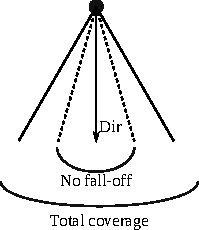
\includegraphics{img/spotlight.pdf}
}
\caption{Spot light geometry.}
\label{FigSpot}
\end{figure}

This light is attenuated based on its distance to the point being
shaded just like a regular point light. For spot attenuation, you can
use the following formula:
%
\begin{align}
s = \left(\frac{\cos(\alpha) -
    \cos(\textrm{falloff}/2)}{\cos(\textrm{falloff}/2)-\cos(\textrm{coverage}/2)}\right)^4,
\end{align}
%
where $\alpha$ is the angle between the light direction and th point
being shaded. The net irradiance at a point $x$ that is $d$ units away
from a spot light is then given by:
%
\begin{align}
E(x) =
\begin{cases}
\frac{I}{d^2} & \textrm{if x is within the no-fall-off zone,} \\
s\frac{I}{d^2} & \textrm{if x is outside the no-fall-off zone but
    inside the coverage zone,} \\
0 & \textrm{otherwise}.
\end{cases}
\end{align}
%
The last type of light that you need to support is the spherical
directional light. This light provides illumination from all angles:
it is an environment light. The radiance values for this light are
defined by an HDR image in latitude-longitude format. Therefore, the
definition of this light uses both a texture element and a light
element. An example is shown below:

\begin{verbatim}
<Textures>
    <Images>
        <Image id="1">textures/pisa_latlong.exr</Image>
    </Images>
</Textures>
<Lights>
    <SphericalDirectionalLight id="1">
        <ImageId>1</ImageId>
    </SphericalDirectionalLight>
</Lights>
\end{verbatim}

To support this light, you need to sample a random direction $d = (x, y, z)$ from the
upper hemisphere of the surface. You can use random rejection sampling
for this purpose (do not worry if your results are a bit noisier than
the provided images at this point). Once a direction is chosen (make
sure that it is a unit vector), you need to convert it to $(u,v)$
values and look up the corresponding value in the HDR environment map. 
You can use the following formula for this purpose:
%
\begin{align}
u &= \frac{1 + \frac{\textrm{atan2}(d_x, d_{-z})}{\pi}}{2}, \\
v &= \frac{\textrm{acos}(d_y)}{\pi}, \\
L(d) &= I(u, v),
\end{align}
%
where $I$ represent the HDR environment map.
As with area lights, you need to compensate for the fact that you
sampled a single direction for illumination. This is done by dividing
the fetched radiance value by the probability density of selecting that
particular direction. Because we sample a random direction uniformly,
this probability density is equal to $p(d) = 1/(2\pi)$. Thus the
overall radiance estimate is computed by:
%
\begin{align}
\hat{L} = \frac{L(d)}{1/(2\pi)} = 2\pi L(d)
\end{align}
%
Note that some spectacular results can be obtained by using this
technique. Figure~\ref{FigAudi} shows two renderings of the same
scene with different environment maps. The appearance of the car model
changes entirely as if it is physically present in different scenes.
Achieving such a result with point lights could be very difficult, if
not impossible.

\begin{figure}
\centerline{
    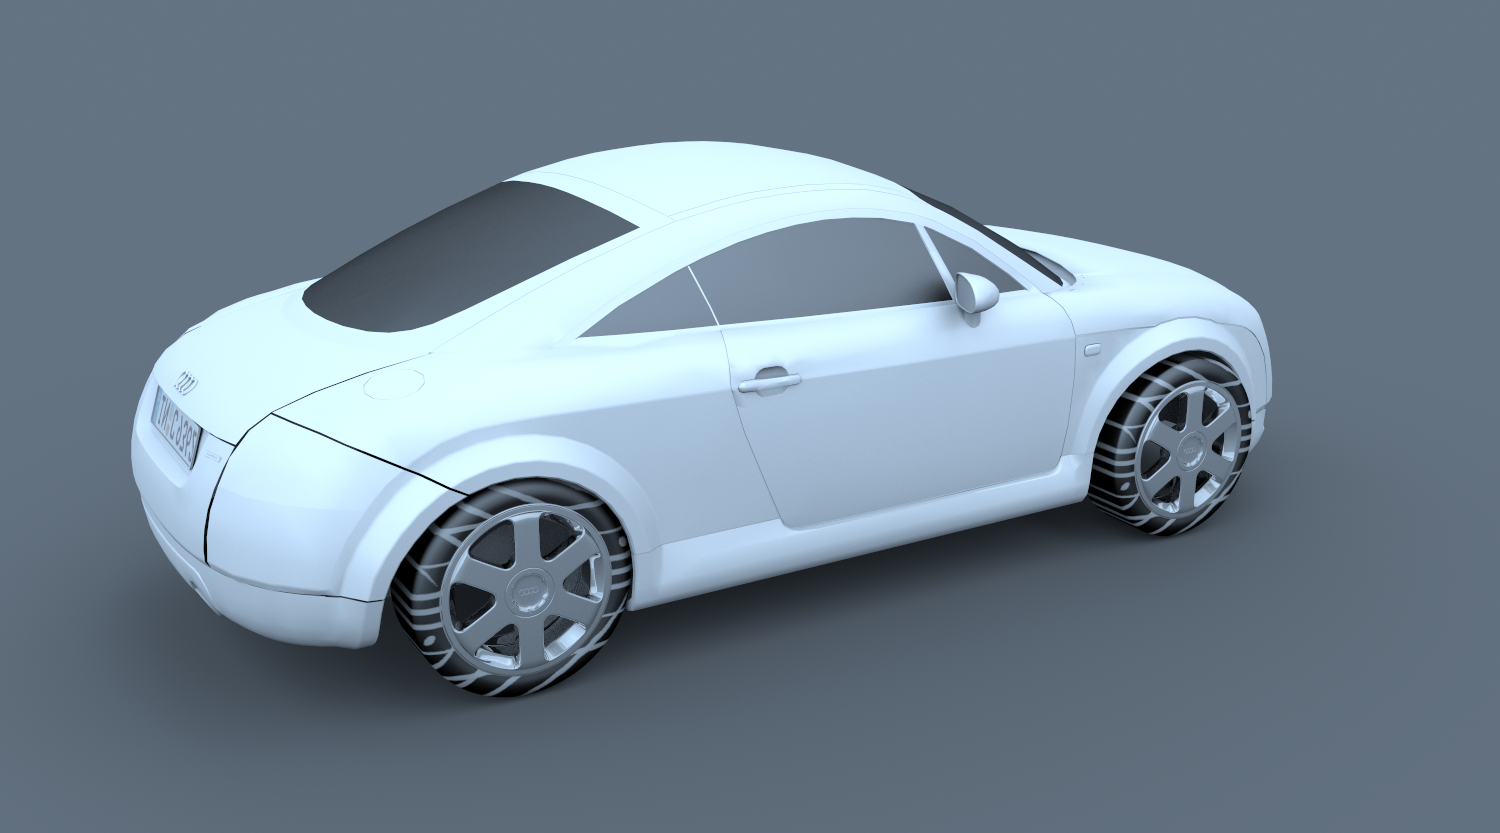
\includegraphics[width=0.48\textwidth]{img/audi-tt-glacier-1600.png}
    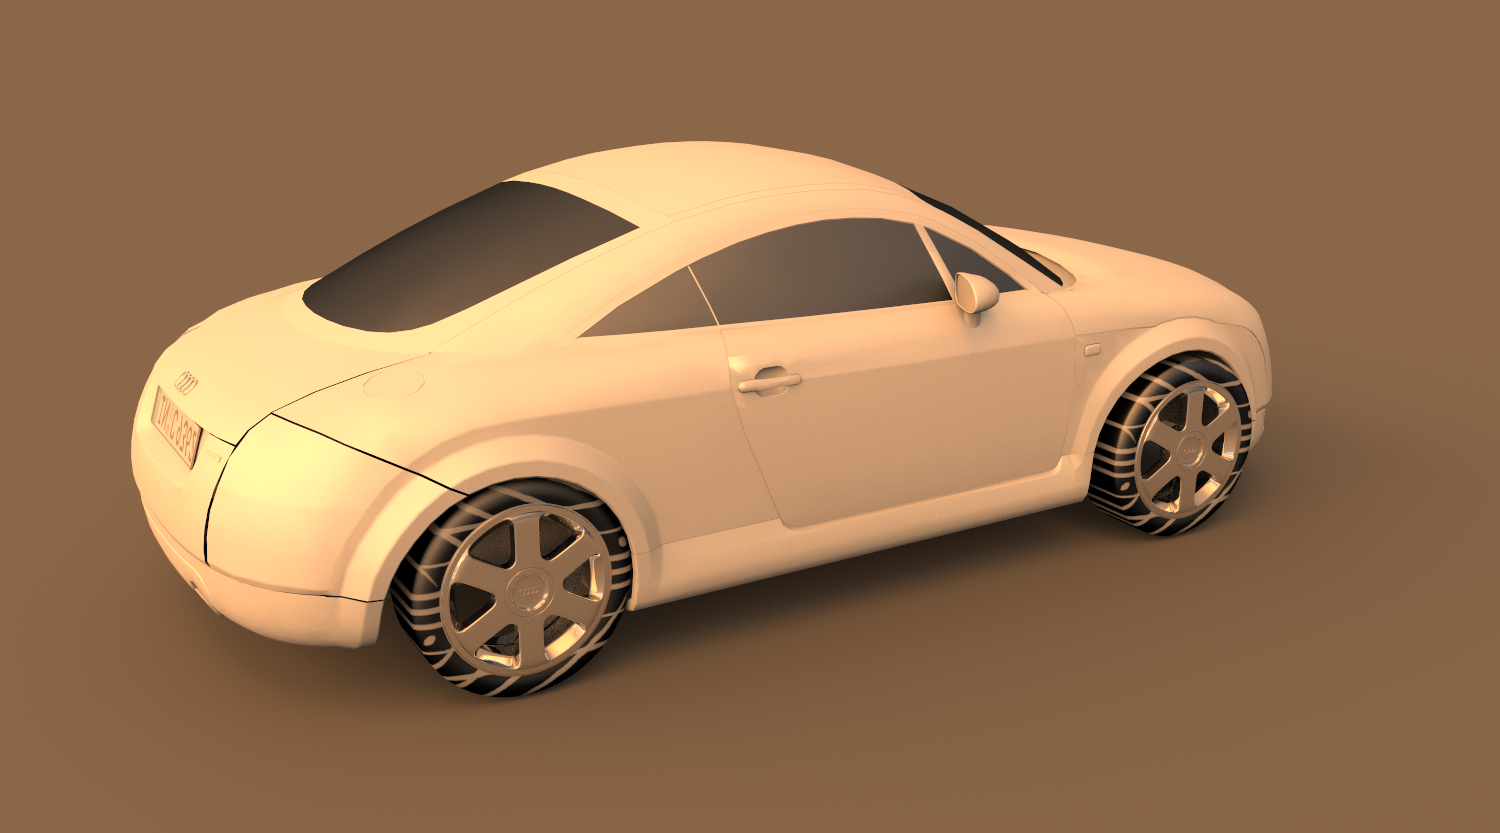
\includegraphics[width=0.48\textwidth]{img/audi-tt-pisa-1600.png}
}
\caption{The same car model is illuminated by different environment
    maps giving rise to very different appearances.}
\label{FigAudi}
\end{figure}

\section{Hints \& Tips}
In addition to those for the previous homeworks, the following tips may
be useful for this homework.

\begin{enumerate}

\item There are a few scenes among the input files that
will make you grateful for having implemented an acceleration
structure, but regretful that you haven't optimized it further.

\item The car model has a few degenerate triangles in some PLY files.
I used to clean such triangles in the past, but it is important that
you can ignore them in your own ray tracers as advanced scenes
generally have such cases. When you insert a triangle to a mesh,
you can simply ignore that triangle if at least any two vertices of
the triangle have the same position.

\item As the car model has some intentional cracks between different
parts of the car, it is a good idea to render this model without
backface culling as otherwise you will see through the car between
these cracks.


\end{enumerate}

\section{Bonus}

I will be more than happy to give bonus points to students who
make important contributions such as new scenes, importers/exporters
between our XML format and other standard file formats. Note that a
Blender
exporter\footnote{\url{https://saksagan.ceng.metu.edu.tr/courses/ceng477/student/ceng477exporter.py}},
which exports Blender data to our XML format, was written by one of our
previous students. You can use this for designing a scene in Blender and
exporting it to our file format.

\section{Regulations}

\begin{enumerate}

\item \textbf{Programming Language:} C/C++ is the recommended language.
However, other languages can be used if so desired. In the past, some
some students used Rust or even Haskell for implementing their ray
tracers.

\item \textbf{Changing the Sample Codes:} You are free to modify any
sample code provided with this homework.

\item \textbf{Additional Libraries:} If you are planning to use any
library other than \textit{(i)} the standard library of the language,
\textit{(ii)} pthread, \textit{(iii)} the XML parser, and the PNG
libraries please first ask about
it on ODTUClass and get a confirmation. Common sense rules apply: if a
library implements a ray tracing concept that you should be
implementing yourself, do not use it!

\item \textbf{Submission:} Submission will be done via ODTUClass. 
To submit, Create a
``\textbf{tar.gz}''  file  named  ``raytracer.tar.gz'' that
contains all your source code files and a Makefile. The
executable should  be  named as  ``raytracer'' and  should  be
able  to  be  run  using  the following commands (scene.xml
        will be provided by us during grading):\\

\indent \textbf{tar -xf raytracer.tar.gz}\\
\indent \textbf{make}\\
\indent \textbf{./raytracer scene.xml}\\

\noindent Any error in these steps will cause point penalty during
grading.

\item \textbf{Late Submission:} You can submit your codes up to 3 days
late. Each late day will cause a 10 point penalty.

\item \textbf{Cheating:} \textbf{We have zero tolerance policy
for cheating}.  People involved in cheating will be
punished according to the university regulations and will
get 0 from the homework. You can discuss algorithmic choices,
but sharing code between groups or using third party code
is strictly forbidden. By the nature of this class, many past students
make their ray tracers publicly available. You must refrain from using
them at all costs.

\item \textbf{Forum:} Check the ODTUClass forum regularly for
updates/discussions.

\item \textbf{Evaluation:} The basis of evaluation is your blog posts.
Please try to create interesting and informative blog posts about your
ray tracing adventures. You can check out various past blogs for
inspiration. However, also expect your codes to be compiled and tested
on some examples for verification purposes. So the images that you share
in your blog post must directly correspond to your ray tracer outputs.

\end{enumerate}

\end{document}
